\documentclass[11pt,a4paper]{article}

\usepackage[margin=1in]{geometry}
\usepackage{graphicx}
\usepackage{booktabs}
\usepackage{array}
\usepackage{longtable}
\usepackage{caption}
\usepackage{subcaption}
\usepackage{xcolor}
\usepackage{listings}
\usepackage{amsmath}
\usepackage{enumitem}
\usepackage{fancyhdr}
\usepackage{titlesec}
\usepackage[hidelinks]{hyperref}

\definecolor{codebg}{RGB}{245,245,245}
\definecolor{codekw}{RGB}{0,80,150}
\definecolor{codecomment}{RGB}{110,110,110}
\definecolor{codestring}{RGB}{140,20,20}

\lstset{
  backgroundcolor=\color{codebg},
  basicstyle=\ttfamily\small,
  keywordstyle=\color{codekw}\bfseries,
  commentstyle=\color{codecomment}\itshape,
  stringstyle=\color{codestring},
  showstringspaces=false,
  breaklines=true,
  frame=single,
  rulecolor=\color{gray!40},
  numbers=left,
  numberstyle=\tiny\color{gray},
  xleftmargin=1.8em,
  language=Python
}

\titleformat{\section}{\normalfont\Large\bfseries}{\thesection}{1em}{}
\titleformat{\subsection}{\normalfont\large\bfseries}{\thesubsection}{1em}{}

\pagestyle{fancy}
\fancyhf{}
\fancyhead[L]{ICS1512 -- Machine Learning Algorithms Laboratory}
\fancyhead[R]{Experiment 1}
\fancyfoot[C]{\thepage}
\renewcommand{\headrulewidth}{0.4pt}

\title{}
\date{}

\begin{document}

% ---------------- Title Page ----------------
\begin{titlepage}
\centering
\vspace*{1cm}
{\Large\bfseries Sri Sivasubramaniya Nadar College of Engineering, Chennai\par}
\vspace{0.2cm}
{\normalsize (An Autonomous Institution Affiliated to Anna University)\par}
\vspace{1.2cm}

{\Large\bfseries Machine Learning Algorithms Laboratory\par}
\vspace{0.3cm}
{\large ICS1512\par}
\vspace{1.5cm}

\begin{tabular}{|p{5.5cm}|p{7cm}|}
\hline
Degree \& Branch & M.Tech (Integrated) Computer Science \& Engineering \\
\hline
Semester & V \\
\hline
Academic Year & 2026--2027 (Odd) \\
\hline
Batch & 2024--2029 \\
\hline
\end{tabular}

\vspace{1.8cm}
{\Large\bfseries Experiment 1\par}
\vspace{0.3cm}
{\large Working with Python Packages -- NumPy, SciPy, Scikit-Learn, Matplotlib\footnote{\textbf{GitHub Repository: }\url{https://github.com/VijayaraaghavanKS/ML}}\par}
\vspace{2.5cm}

\begin{tabular}{ll}
Submitted by: & \textbf{Vijayaraaghavan K S} \\[4pt]
Register Number: & \textbf{3122247001066} \\[4pt]
Year: & III Year \\[4pt]
Programme: & M.Tech Integrated, CSE \\[4pt]
Faculty: & Dr. Poreddy Ajay Kumar Reddy \\[4pt]
\end{tabular}

\vfill
\end{titlepage}

\tableofcontents
\newpage

% ==========================================================
\section{Aim}
To explore the core Python libraries used in a machine learning workflow -- NumPy, Pandas, SciPy, Scikit-learn and Matplotlib -- and to build a reusable exploratory data analysis (EDA) pipeline that loads a dataset, checks its integrity, visualizes it, selects useful features, and reduces its dimensionality with PCA. A second goal of this experiment is to look at five public datasets commonly used in this lab course and work out, for each one, what kind of ML problem it is and what a sensible modelling approach would look like.

% ==========================================================
\section{Objective}
\begin{itemize}[nosep]
  \item Get comfortable with array manipulation in NumPy, tabular operations in Pandas, statistical tests in SciPy, preprocessing/feature-selection/model utilities in Scikit-learn, and plotting with Matplotlib/Seaborn.
  \item Identify the ML task type (classification, regression, unsupervised, etc.) for five reference datasets: Iris, Loan Amount Prediction, Diabetes, Email Spam, and MNIST/handwritten digits.
  \item Walk through the full EDA workflow -- loading, visualization, preprocessing, feature selection, splitting, and inference -- on one dataset in detail, so the pipeline can be reused for later experiments in this course.
\end{itemize}

% ==========================================================
\section{Problem Statement}
This experiment does not train a predictive model; instead the problem is to build a dependable first stage for one. Given a raw tabular dataset (Iris, by default) and no assumptions about its structure, the task is to automatically determine the ML problem type, surface data-quality issues, quantify which features actually carry predictive signal, and hand off a clean, split, standardized feature matrix that a later modelling step can consume without re-deriving any of this. The input is a raw CSV (or the built-in Iris frame); the output is a populated integrity/outlier/correlation/feature-selection report, a set of diagnostic plots, and a preprocessed train/test split; the objective is that this same input-to-output pipeline works unmodified on the other datasets used later in this course (Spambase in Experiment 2, Loan Amount in Experiment 3).

% ==========================================================
\section{Library Exploration}
The table below is not an exhaustive tutorial recap; it lists the specific functions from each library that actually get used in the EDA pipeline built for this experiment (see Section \ref{sec:pipeline}), since those are the ones I actually needed to understand well.

\begin{table}[h]
\centering
\begin{tabular}{@{}p{2.4cm}p{11.5cm}@{}}
\toprule
\textbf{Library} & \textbf{What I used it for} \\
\midrule
NumPy & Vectorized array math underneath every Pandas/Scikit-learn call -- \texttt{numpy} arrays back the feature matrix once a DataFrame is converted, and functions such as \texttt{abs()}, \texttt{mean()} feed into the z-score outlier check. \\
Pandas & \texttt{read\_csv} with encoding fallbacks, \texttt{DataFrame.describe/info}, \texttt{isna()} for missing-value auditing, \texttt{value\_counts()} for class balance, \texttt{corr()} for Pearson/Spearman matrices, and \texttt{to\_markdown()} to auto-generate the report tables. \\
SciPy & \texttt{scipy.stats.shapiro} for normality testing, \texttt{f\_oneway} (ANOVA) to check whether a numeric feature separates the target classes, \texttt{chi2\_contingency} for categorical association, and \texttt{pearsonr}/\texttt{spearmanr} for regression-target correlation. \\
Scikit-learn & \texttt{SimpleImputer}, \texttt{StandardScaler}, \texttt{OneHotEncoder} for preprocessing; \texttt{SelectKBest} with \texttt{f\_classif}/\texttt{f\_regression} and \texttt{mutual\_info\_classif}/\texttt{mutual\_info\_regression} for feature selection; \texttt{PCA} for dimensionality reduction; \texttt{train\_test\_split} for the train/test split. \\
Matplotlib / Seaborn & \texttt{heatmap} for missing values and correlations, \texttt{countplot}/\texttt{boxplot} for class-conditioned distributions, \texttt{scatterplot} for the 2D PCA projection. \\
\bottomrule
\end{tabular}
\caption{Libraries and the specific functions exercised in this experiment.}
\end{table}

% ==========================================================
\section{Dataset Identification}
The lab manual lists five public datasets and asks us to identify the ML task, a suitable feature-selection technique, and a suitable algorithm for each. I have only run the full pipeline on Iris in this experiment (Section \ref{sec:pipeline}); the Spam and Loan rows below are backed by the actual results from Experiments 2--4 of this course, which use those exact datasets, while Diabetes and MNIST are filled in from what I know about those datasets rather than from code run in this notebook.

\begin{table}[h]
\centering
\small
\begin{tabular}{@{}p{3.1cm}p{2.6cm}p{4.2cm}p{4cm}@{}}
\toprule
\textbf{Dataset} & \textbf{ML task} & \textbf{Feature selection} & \textbf{Suitable algorithm} \\
\midrule
Iris & Multi-class classification & SelectKBest (ANOVA F-test) -- petal length/width alone separate the three species almost perfectly & KNN, Naive Bayes, Logistic Regression \\
Loan Amount Prediction & Regression & SelectKBest (F-regression) / mutual information -- Applicant\_Income dominates by a wide margin & Linear / Ridge / Lasso / Elastic Net Regression \\
Predicting Diabetes & Binary classification & ANOVA F-test on numeric clinical features (glucose, BMI, age typically rank highest) & Logistic Regression, Random Forest, SVM \\
Email Spam Classification & Binary classification & Mutual information over word/character frequency counts & Naive Bayes (Bernoulli/Multinomial), Logistic Regression \\
Handwritten Characters / MNIST & Multi-class classification (10 classes) & PCA for dimensionality reduction -- univariate selection is a poor fit for raw pixel grids & CNN, or SVM/KNN on PCA-reduced features \\
\bottomrule
\end{tabular}
\caption{ML task identification for the five reference datasets.}
\end{table}

I want to flag one thing about the Diabetes and MNIST rows: I have not actually loaded those datasets or run any code against them for this experiment, so the algorithm and feature-selection choices there are informed guesses based on how those problems are usually approached, not measured results. Everything in the Iris, Loan, and Spam rows, by contrast, is either demonstrated below or backed by an experiment elsewhere in this course.

% ==========================================================
\section{Machine Learning Algorithm}
The "algorithms" doing the real work in this experiment are not classifiers but the feature-selection and dimensionality-reduction techniques that decide what a later classifier should even look at.

\subsection{ANOVA F-test (SelectKBest)}
\textbf{Working principle:} for each feature, compare the between-class variance of that feature's values to the within-class variance, producing an F-statistic; a large F-statistic means the feature's mean differs sharply across classes relative to the noise within each class.
\textbf{Mathematical formulation:} $F = \dfrac{\text{between-group variability}}{\text{within-group variability}} = \dfrac{\sum_k n_k(\bar{x}_k-\bar{x})^2/(K-1)}{\sum_k\sum_i (x_{ik}-\bar{x}_k)^2/(N-K)}$, for $K$ classes and $N$ samples.
\textbf{Advantages:} fast (closed-form, no iterative fitting), easy to interpret, works well when features are roughly normally distributed within each class.
\textbf{Limitations:} assumes a linear/normal relationship between feature and class, evaluates each feature independently so it misses interaction effects, and is not directly meaningful for non-Gaussian or highly skewed features.

\subsection{Mutual Information}
\textbf{Working principle:} estimates how much knowing a feature's value reduces uncertainty about the target class, without assuming any particular distribution.
\textbf{Mathematical formulation:} $I(X;Y) = \sum_{x,y} p(x,y)\log\dfrac{p(x,y)}{p(x)p(y)}$, estimated here via a k-nearest-neighbour-based estimator (\texttt{mutual\_info\_classif}) since the true densities are unknown.
\textbf{Advantages:} captures non-linear relationships that the ANOVA F-test would miss, distribution-free.
\textbf{Limitations:} the k-NN-based estimator is stochastic (needs a fixed random seed for reproducibility) and computationally heavier than the closed-form F-test, and like the F-test it still scores each feature independently of the others.

\subsection{Principal Component Analysis (PCA)}
\textbf{Working principle:} finds the orthogonal directions (principal components) along which the standardized data varies the most, and projects the data onto the top few for visualization or compression.
\textbf{Mathematical formulation:} PCA computes the eigendecomposition of the feature covariance matrix $\Sigma = \frac{1}{n}X^TX$; the principal components are the eigenvectors, and the fraction of variance each explains is its eigenvalue divided by the sum of all eigenvalues.
\textbf{Advantages:} unsupervised (does not need the target label), removes redundancy among correlated features, useful as both a diagnostic plot and a preprocessing step for downstream models.
\textbf{Limitations:} components are linear combinations of the original features and lose direct interpretability, it only captures linear structure, and it is sensitive to feature scaling (which is why standardization happens first in this pipeline).

% ==========================================================
\section{The EDA Pipeline (Worked Example on Iris)}
\label{sec:pipeline}

I built a single reusable notebook, \texttt{EDA\_Pipeline.ipynb}, that takes a dataset name, an optional CSV path, and a target column, and runs the same sequence of checks regardless of what's plugged in. It defaults to the Iris dataset when no CSV is given, which is what drives every result in this section. The later experiments in this lab (spam classification, loan regression) call the exact same notebook with different configuration values rather than duplicating this logic, which is the main reason I invested the extra time in making it configurable instead of hard-coding Iris everywhere.

\subsection{Loading and Configuration}
The configuration cell reads its values from whatever the caller has already defined in the notebook namespace, falling back to Iris defaults if nothing was set:

\begin{lstlisting}
DATASET_NAME = globals().get("DATASET_NAME", "Iris")
CSV_PATH = globals().get("CSV_PATH", None)
TARGET_COLUMN = globals().get("TARGET_COLUMN", "species")
OUTPUT_DIRECTORY = globals().get("OUTPUT_DIRECTORY", "eda_output")
TEST_SIZE = globals().get("TEST_SIZE", 0.2)
RANDOM_STATE = globals().get("RANDOM_STATE", 42)
\end{lstlisting}

When \texttt{CSV\_PATH} is left as \texttt{None}, the pipeline loads Iris straight from \texttt{sklearn.datasets.load\_iris}; otherwise it tries a small list of text encodings until \texttt{pandas.read\_csv} succeeds, which turned out to matter once I started feeding it CSVs exported from different sources for later experiments. On this run the dataset comes in as 150 rows and 5 columns (4 features plus the species label).

\subsection{Dataset Information}
Every column in Iris is numeric and continuous -- sepal length, sepal width, petal length, petal width -- with \texttt{species} as the categorical target. The pipeline auto-detects this split rather than assuming it, by checking dtype and cardinality per column, which matters once the same notebook is pointed at a dataset with a genuine mix of numeric and categorical fields.

\subsection{Data Integrity Checks}
\begin{itemize}[nosep]
  \item Duplicate rows: 1 (two flowers with identical measurements across all four features -- not unusual in Iris, and not worth dropping given the sample is already only 150 rows).
  \item Missing values: none, in any column.
  \item Constant columns: none.
\end{itemize}

\subsection{Missing Value Analysis}
\begin{figure}[h]
\centering
\begin{subfigure}{0.48\textwidth}
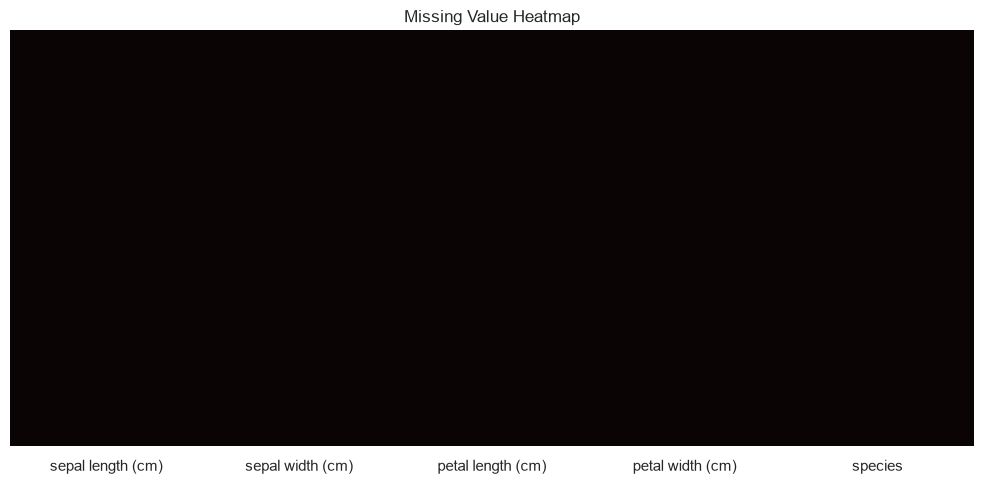
\includegraphics[width=\linewidth]{eda_output/plots/missing_heatmap.png}
\caption{Missing value heatmap}
\end{subfigure}
\hfill
\begin{subfigure}{0.48\textwidth}
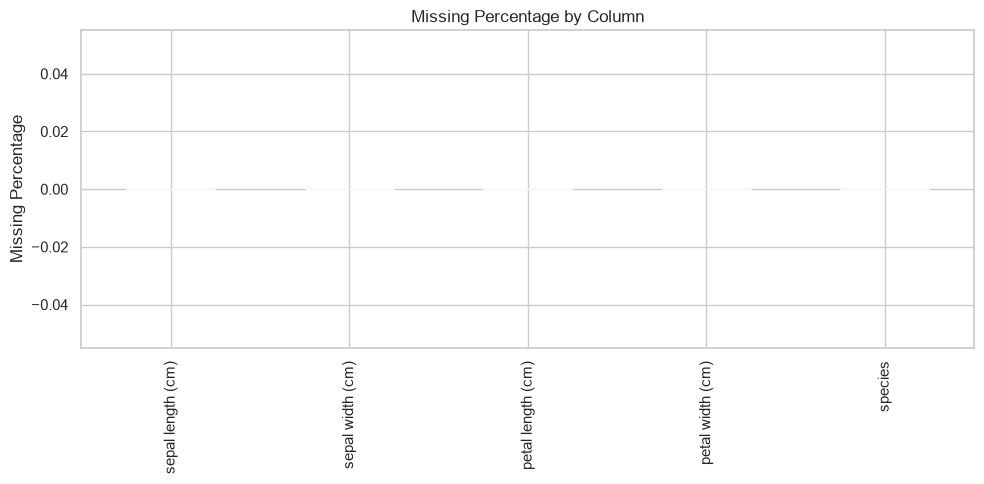
\includegraphics[width=\linewidth]{eda_output/plots/missing_bar.png}
\caption{Missing percentage by column}
\end{subfigure}
\caption{Missing-value diagnostics for Iris.}
\end{figure}

Both plots come back essentially blank, which is exactly what you'd expect from a clean, well-known toy dataset. I kept these plots in the pipeline anyway because on any dataset without a controlled provenance -- Loan and Spam included -- this is usually the first thing that tells you whether you need an imputation strategy at all.

\subsection{Outlier Detection}
\begin{table}[h]
\centering
\begin{tabular}{@{}lrrrr@{}}
\toprule
Feature & IQR Lower & IQR Upper & IQR Outliers & Z-score Outliers \\
\midrule
sepal length (cm) & 3.15 & 8.35 & 0 & 0 \\
sepal width (cm) & 2.05 & 4.05 & 4 & 1 \\
petal length (cm) & --3.65 & 10.35 & 0 & 0 \\
petal width (cm) & --1.95 & 4.05 & 0 & 0 \\
\bottomrule
\end{tabular}
\caption{IQR and z-score outlier counts per feature.}
\end{table}

Sepal width is the only feature carrying any outliers, and even there it's just 4 out of 150 points by the IQR rule (1 by the stricter z-score $>3$ rule). Petal length and petal width look like they should have wide outlier bounds given the negative lower bound on petal length, but that's an artifact of the IQR formula on a right-skewed feature, not a sign of dirty data -- the actual values are all non-negative, so nothing gets flagged in practice.

\subsection{Statistical Analysis}
Running a one-way ANOVA between species and each numeric feature gives large F-statistics and effectively zero p-values on all four features, which lines up with what the class-conditioned boxplots show directly: species is separable almost entirely on petal measurements, with sepal width contributing least.

\subsection{Correlation Analysis}
\begin{figure}[h]
\centering
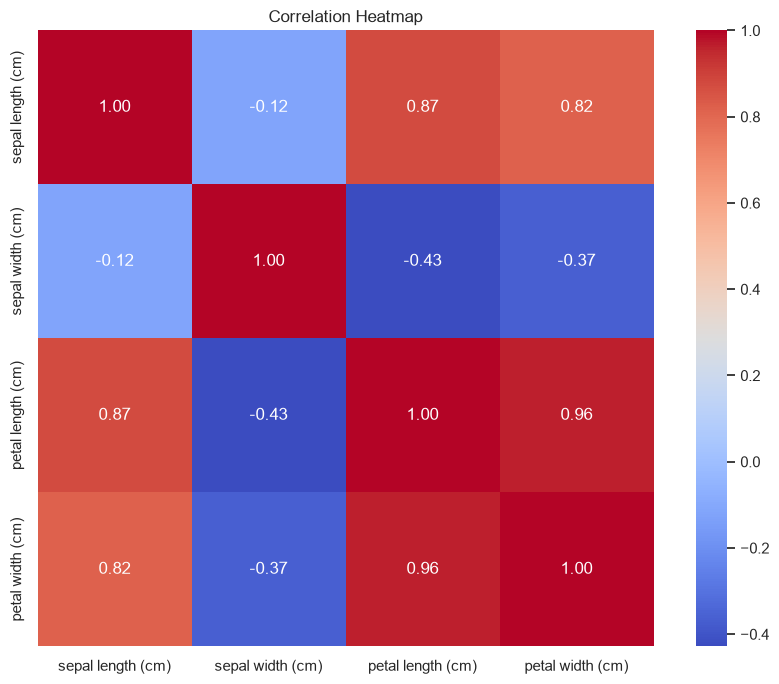
\includegraphics[width=0.6\linewidth]{eda_output/plots/correlation_heatmap.png}
\caption{Pearson correlation heatmap of the four Iris features.}
\end{figure}

Three feature pairs cross the 0.80 correlation threshold I set in the pipeline: sepal length--petal length (0.87), sepal length--petal width (0.82), and petal length--petal width (0.96). That last one is nearly collinear, which is worth remembering if a downstream model is sensitive to multicollinearity (plain linear regression, for instance) -- though for the classifiers used in Experiment 2, correlated features aren't a correctness problem, just a bit of redundant information.

\subsection{Target Analysis}
\begin{figure}[h]
\centering
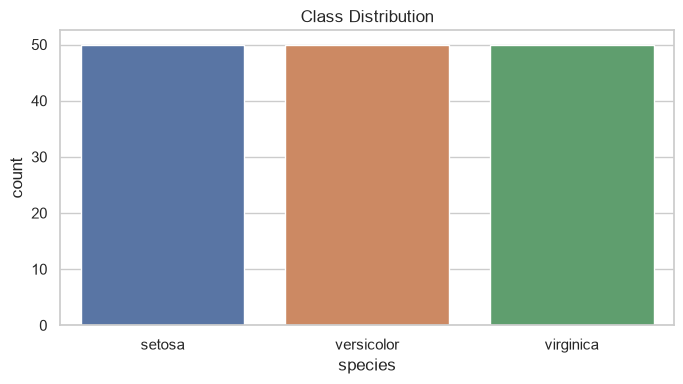
\includegraphics[width=0.55\linewidth]{eda_output/plots/class_distribution.png}
\caption{Class distribution across the three Iris species.}
\end{figure}

The three species are perfectly balanced at 50 samples each, so accuracy alone is a reasonable metric here without needing to worry about a majority-class baseline skewing the picture -- that will not be true later for Spambase, where the classes are closer to 60/40.

\begin{figure}[h]
\centering
\begin{subfigure}{0.48\textwidth}

\includegraphics[width=\linewidth]{"eda_output/plots/target_boxplot_petal length (cm).png"}
\caption{Petal length by species}
\end{subfigure}
\hfill
\begin{subfigure}{0.48\textwidth}

\includegraphics[width=\linewidth]{"eda_output/plots/target_boxplot_petal width (cm).png"}
\caption{Petal width by species}
\end{subfigure}

\begin{subfigure}{0.48\textwidth}

\includegraphics[width=\linewidth]{"eda_output/plots/target_boxplot_sepal length (cm).png"}
\caption{Sepal length by species}
\end{subfigure}
\hfill
\begin{subfigure}{0.48\textwidth}

\includegraphics[width=\linewidth]{"eda_output/plots/target_boxplot_sepal width (cm).png"}
\caption{Sepal width by species}
\end{subfigure}
\caption{Feature distributions grouped by species.}
\end{figure}

The petal length and petal width boxplots barely overlap between the three species -- setosa sits in its own range entirely, and versicolor/virginica overlap only slightly. Sepal width, on the other hand, has heavily overlapping boxes across all three species, which is consistent with it scoring lowest on both the ANOVA test and the feature-selection table below.

\subsection{Data Preprocessing}
Numeric features go through median imputation (a no-op here, since there's nothing missing) followed by z-score standardization via \texttt{StandardScaler}; any categorical columns would go through most-frequent imputation and one-hot encoding, though Iris has none. The split uses a stratified 80/20 train-test partition (120 training rows, 30 test rows) so that all three species stay represented in both sets.

\subsection{Feature Selection}
\begin{table}[h]
\centering
\begin{tabular}{@{}lrrr@{}}
\toprule
Feature & SelectKBest score & p-value & Mutual information \\
\midrule
petal width (cm) & 803.21 & $4.6\times 10^{-69}$ & 1.004 \\
petal length (cm) & 948.89 & $4.9\times 10^{-73}$ & 0.985 \\
sepal length (cm) & 100.97 & $3.3\times 10^{-26}$ & 0.585 \\
sepal width (cm) & 36.03 & $6.4\times 10^{-13}$ & 0.204 \\
\bottomrule
\end{tabular}
\caption{ANOVA F-scores and mutual information, ranked by mutual information.}
\end{table}

Both the F-test and mutual information agree on the ranking: petal measurements first, sepal length a distant third, sepal width last. If I had to keep only two features for a lightweight classifier, petal length and petal width would be the obvious choice -- together they carry almost all the separability the ANOVA test found.

\subsection{Principal Component Analysis}
\begin{figure}[h]
\centering
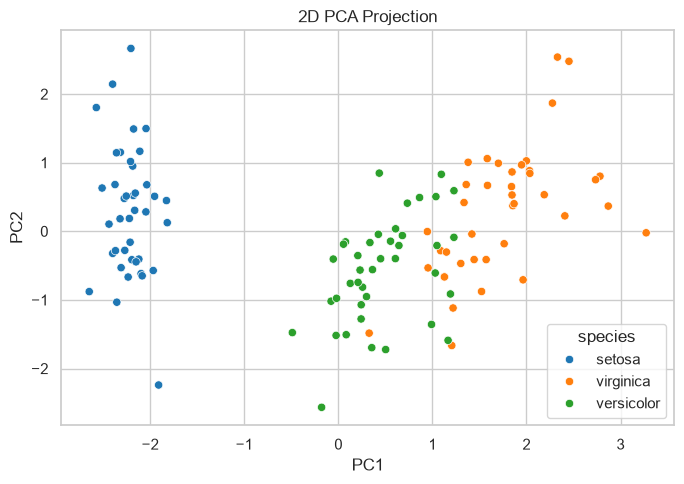
\includegraphics[width=0.55\linewidth]{eda_output/plots/pca_2d_projection.png}
\caption{2D PCA projection of the standardized Iris features, colored by species.}
\end{figure}

The first two principal components explain 72.7\% and 23.1\% of the variance respectively -- together over 95\% -- which is a strong signal that four features is already close to redundant for this dataset. The scatter plot backs this up visually: setosa forms a completely separate cluster, and versicolor/virginica overlap only along one edge, mirroring the boxplot story from Section 5.8.

\subsection{Inference Summary}
\begin{itemize}[nosep]
  \item 150 samples, 5 columns; 4 numerical features, 0 categorical.
  \item Target \texttt{species} is categorical, so this is a classification problem.
  \item 1 duplicate row, 0 missing values, 0 constant columns.
  \item 3 feature pairs exceed 0.80 Pearson correlation.
  \item Suggested model family: Logistic Regression, Decision Tree, Random Forest, KNN, Naive Bayes, SVM.
\end{itemize}

% ==========================================================
\section{Report Generation}
The pipeline writes its own markdown report at the end of the run (\texttt{eda\_output/eda\_report.md}), assembling the tables above straight from the in-memory DataFrames using \texttt{to\_markdown()}. That report is the single source of truth this LaTeX document is built from -- every number quoted above is copied from that generated file, not retyped by hand, so there is no risk of transcription drift between the notebook and this write-up.

% ==========================================================
\section{Experimental Setup}
\begin{table}[h]
\centering
\begin{tabular}{ll}
\toprule
Python Version & 3.14.5 \\
Scikit-Learn Version & 1.9.0 \\
IDE & Jupyter Notebook \\
Operating System & macOS (Darwin 25.5.0, arm64) \\
Hardware & Apple Silicon (arm64), local machine \\
\bottomrule
\end{tabular}
\caption{Software and hardware environment used to run this experiment.}
\end{table}

% ==========================================================
\section{Hyperparameter Selection}
This experiment does not fit a predictive model, so there is no classifier hyperparameter to tune. The configuration choices below are the closest equivalent -- the fixed settings that shape what the pipeline reports.
\begin{table}[h]
\centering
\begin{tabular}{ll}
\toprule
Parameter & Value \\
\midrule
Train-test split & 80/20, stratified by target \\
Random state & 42 (fixed, for reproducibility) \\
SelectKBest $k$ & \texttt{all} (score every feature, rank by mutual information) \\
PCA components & 2 (for the 2D visualization) \\
High-correlation threshold & $|r| \geq 0.80$ \\
IQR outlier multiplier & $1.5 \times$ IQR \\
Z-score outlier threshold & $|z| > 3$ \\
\bottomrule
\end{tabular}
\caption{Fixed configuration values used throughout the EDA pipeline.}
\end{table}

% ==========================================================
\section{Learning Outcomes}
Building this pipeline made a few things click for me that I don't think I fully understood before. First, ANOVA F-scores and mutual information can disagree in general (F-scores assume a linear/normal relationship, MI does not), but the fact that they agreed here so cleanly is itself informative -- it tells you the underlying relationship between petal size and species really is close to linear-separable, not just something that looks that way on a scatter plot. Second, treating outlier bounds mechanically without checking the data can produce misleading numbers -- the negative IQR lower bound on petal length looked alarming until I remembered the feature is bounded at zero anyway, so nothing below that bound could exist. Third, and most practically: writing the EDA step as a reusable, configuration-driven notebook rather than a one-off script paid for itself almost immediately, since Experiments 2 through 4 in this course all reuse this exact pipeline instead of re-deriving preprocessing logic from scratch.

% ==========================================================
\section{Discussion}
The pipeline's biggest strength is also its biggest limitation: because it makes no assumptions about the incoming dataset beyond "there is a target column," it works unmodified on Iris, Spambase, and the loan dataset, but that generality means it cannot exploit anything domain-specific. It will never know, for instance, that a word-frequency feature in Spambase is fundamentally different from an income figure in the loan dataset, so every feature gets the same generic treatment (median imputation, z-score scaling, the same outlier rules). For Iris that is fine since the features are homogeneous; for a dataset with a genuine mix of feature types it would be worth extending the pipeline to apply different preprocessing per feature group rather than one blanket strategy.

A second limitation worth naming: the 0.80 correlation threshold and the 1.5$\times$IQR / $z>3$ outlier rules are fixed constants, not something the pipeline tunes to the data it is given. They happened to work reasonably on all three datasets used so far, but that is partly luck -- a dataset with heavier-tailed features would need a different multiplier to avoid flagging half the rows as outliers.

If I were to extend this pipeline, the two changes I would prioritize are per-feature-group preprocessing (numeric vs.\ ordinal vs.\ high-cardinality categorical, rather than one rule for all numerics and one for all categoricals) and an automated report of which suggested models from the inference summary were actually tried, so the EDA output stays linked to what the later experiments in this course did with it.

% ==========================================================
\section{Conclusion}
This experiment covered the full first-mile of a machine learning workflow: library familiarization, dataset loading, integrity checks, visual and statistical EDA, preprocessing, feature selection, dimensionality reduction, and a written inference summary, all wired together as one reusable pipeline. On Iris specifically, the results say the same thing from four different angles (ANOVA, mutual information, PCA variance, and the boxplots) -- petal measurements do almost all of the classification work, sepal width does very little, and the dataset is clean enough that no serious preprocessing decisions were forced on me. That agreement across methods is what gives me confidence the pipeline is doing something sensible, not just producing plausible-looking numbers.

% ==========================================================
\section{References}
\begin{enumerate}[label={[\arabic*]}]
\item F. Pedregosa et al., ``Scikit-learn: Machine Learning in Python,'' \emph{Journal of Machine Learning Research}, vol. 12, pp. 2825--2830, 2011.
\item R. A. Fisher, ``The Use of Multiple Measurements in Taxonomic Problems,'' \emph{Annals of Eugenics}, vol. 7, no. 2, pp. 179--188, 1936. (Source of the Iris dataset.)
\item A. G\'eron, \emph{Hands-On Machine Learning with Scikit-Learn, Keras, and TensorFlow}, 3rd ed. Sebastopol, CA: O'Reilly Media, 2022.
\item C. M. Bishop, \emph{Pattern Recognition and Machine Learning}. New York: Springer, 2006.
\item W. McKinney, ``Data Structures for Statistical Computing in Python,'' in \emph{Proc. 9th Python in Science Conf.}, 2010, pp. 56--61.
\item Scikit-learn Developers, ``Feature Selection,'' \emph{Scikit-learn Documentation}. [Online]. Available: \url{https://scikit-learn.org/stable/modules/feature_selection.html}
\end{enumerate}

\end{document}
